\chapter{Optimization for Machine Learning}
\chaptermark{Optimization for Machine Learning}
\label{chap:optimization}

In Homework~2, Task~6, we fitted a model by evaluating its loss at 601
parameter values and keeping the best one. With two adjustable parameters,
the same grid would require \(601^2=361{,}201\) evaluations. A derivative
lets us use what happens at the current parameter value to choose the next one.

\section{A gradient step for the homework model}
Two inputs, \(x=1\) and \(x=2\), occur equally often. A teacher assigns
probability \(p_1=0.80\) and \(p_2=0.60\) to class 1. Our student model uses
one parameter \(a\) for both predictions:
\[
  q_a(x)=\sigma(ax),\qquad \sigma(z)=\frac{1}{1+e^{-z}}.
\]
At \(a=\log 4\), the predictions are \(4/5\) and \(16/17\). The first
matches its target exactly. The second is about \(0.94\), well above \(0.60\).
Decreasing \(a\) lowers both predictions. How much does correcting the
second prediction cost us on the first?

Write \(\ell_x(a)\) for the binary cross-entropy on input \(x\).
The two inputs have equal weight, so their mean loss is
\[
 \ell_x(a)=-p_x\log q_a(x)-(1-p_x)\log(1-q_a(x)),\qquad
 L(a)=\tfrac12\bigl(\ell_1(a)+\ell_2(a)\bigr).
\]
As in Chapter~\ref{chap:information}, the teacher entropy is fixed. A change
in this loss therefore equals the change in mean forward KL divergence.

To differentiate, first let \(q=q_a(x)\) and change the predicted
probability while holding its target fixed. Then account for how \(q\)
changes when \(a\) moves:
\[
 \frac{\partial\ell_x}{\partial q}
   =-\frac{p_x}{q}+\frac{1-p_x}{1-q}
   =\frac{q-p_x}{q(1-q)},\qquad
 \frac{dq}{da}=xq(1-q).
\]
\begin{result}[Derivative of the student loss]
The chain rule gives \(\ell'_x(a)=x(q_a(x)-p_x)\).
The full derivative is the average
\(L'(a)=\tfrac12\bigl(\ell'_1(a)+\ell'_2(a)\bigr)\).
\end{result}
For these positive inputs, predicting too much probability for class 1 gives
a positive derivative. A small decrease in \(a\) then reduces that input's
loss. At an exact match the first-order change is zero.

\clearpage
\subsection*{Taking the first step}
At \(a_0=\log 4\), the first derivative contribution is zero and the second
is \(2(16/17-0.60)\approx0.6824\). Their average is \(0.3412\).
The linear approximation \(L(a+h)\approx L(a)+hL'(a)\) explains the
direction of the step. With \(h=-\eta L'(a)\), the predicted change is
\(-\eta[L'(a)]^2\). The approximation describes sufficiently small steps.

\begin{definition}[Gradient descent]
For a differentiable loss \(L\), take a step opposite its gradient:
\[
  w_{k+1}=w_k-\eta\nabla L(w_k).
\]
Here \(k\) counts updates, \(\eta>0\) is the learning rate, and the gradient
collects one partial derivative per parameter. For a single parameter it is
the ordinary derivative.
\end{definition}

Using \(\eta=1\) in the student model gives \(a_1=1.3863-0.3412=1.0451\).
The mean loss falls from \(0.8350\) to \(0.7315\) nats. Repeating the same
calculation gives \(a_2=0.7852\) and \(a_3=0.6140\).

\begin{figure}[H]\centering
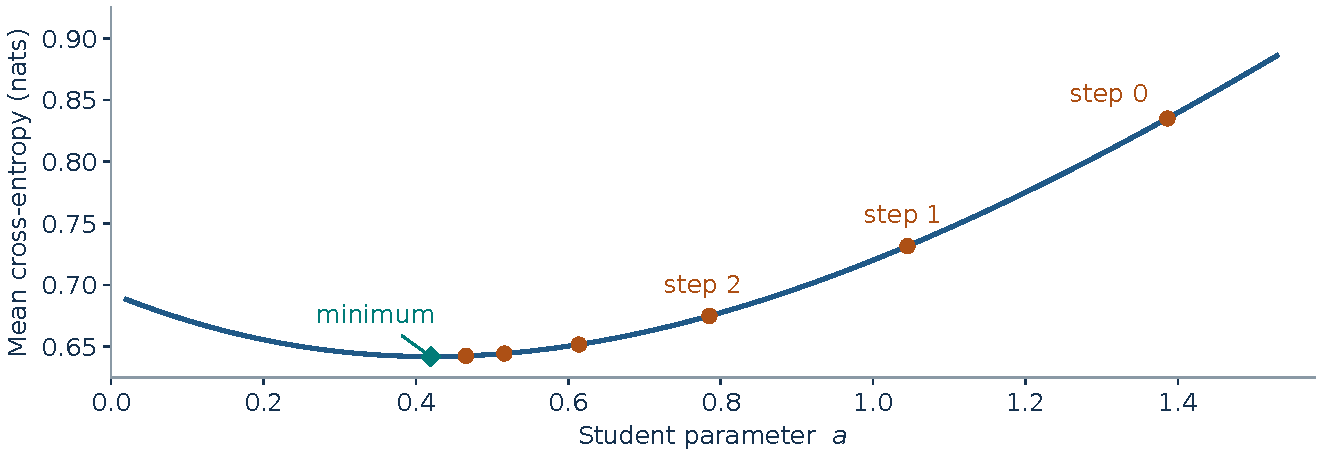
\includegraphics[width=.93\linewidth]{figures/ch8/student-descent.pdf}
\caption{The orange points are gradient updates starting at \(\log 4\).
Their spacing decreases as the derivative approaches zero.}
\end{figure}

Why trust the minimum we see? Differentiating again gives
\(L''(a)=\tfrac12\sum_{x=1,2}x^2q_a(x)(1-q_a(x))>0\) for every finite \(a\).
The slope increases throughout this curve. Its unique zero is
\(a_*\approx0.41962\). The homework grid gives \(0.42086\), close enough
that the two fits look identical at the scale of the figure.

\clearpage
\section{How far can one step go?}
On a quadratic loss \(F(w)=cw^2/2\) with \(c>0\), the minimum is zero at
\(w=0\). The second derivative \(c\) measures curvature. Since \(F'(w)=cw\),
gradient descent multiplies the parameter by the same number at every step:
\[
  w_{k+1}=(1-\eta c)w_k,\qquad w_k=(1-\eta c)^k w_0.
\]
\begin{result}[Stable learning rates on a scalar quadratic]
From any nonzero starting point, \(w_k\to 0\) exactly when
\(\lvert1-\eta c\rvert<1\), or equivalently \(0<\eta<2/c\).
\end{result}
For \(c=1\) and \(w_0=4\), the sign and magnitude of this multiplier explain
five different runs:
\begin{center}
\begin{tabular}{@{}rrll@{}}\toprule
\(\eta\)& \(1-\eta c\)& First three parameter values & Behaviour\\\midrule
0.5 & 0.5 & \(4,\,2,\,1\) & Approaches zero from one side\\
1   & 0   & \(4,\,0,\,0\) & Reaches zero in one step\\
1.5 & \(-0.5\)& \(4,\,-2,\,1\) & Crosses zero and converges\\
2   & \(-1\)& \(4,\,-4,\,4\) & Repeats at constant loss\\
2.5 & \(-1.5\)& \(4,\,-6,\,9\) & Moves farther away\\\bottomrule
\end{tabular}
\end{center}
\begin{figure}[H]\centering
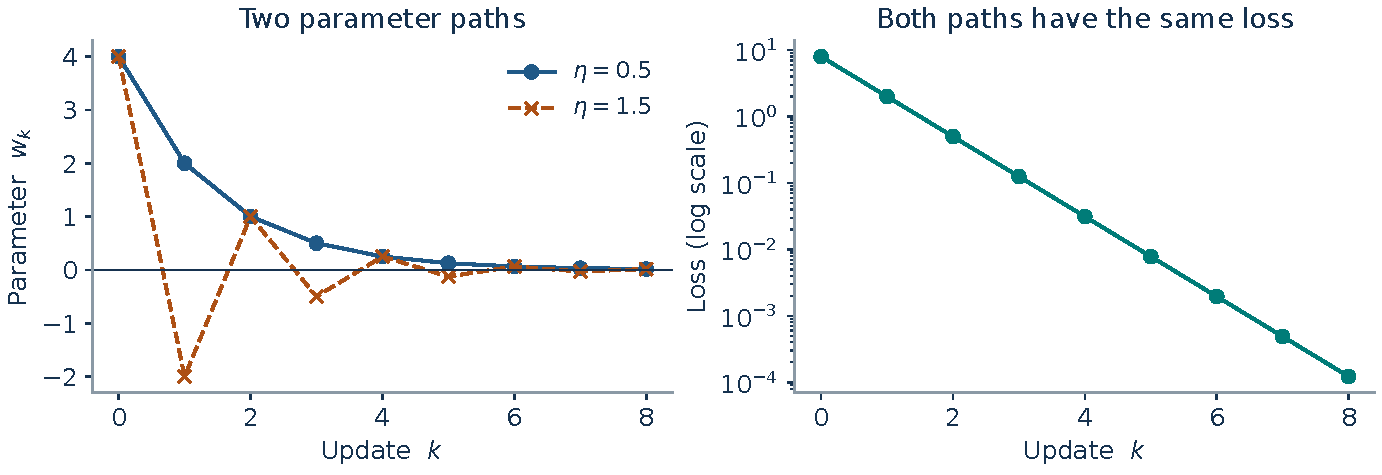
\includegraphics[width=\linewidth]{figures/ch8/parabola.pdf}
\caption{The blue and orange runs have opposite signs on odd updates. Their
squared parameters coincide at every update, so both runs produce the
single loss curve on the right.}
\end{figure}
Section~\ref{sec:observed-information} used curvature to describe the drop
in log-likelihood near its maximum. Here curvature describes how quickly the
slope changes while an optimizer moves. On this parabola, doubling the
curvature halves the upper limit on stable step sizes.

\clearpage
\section{A steep direction can slow a flat one}
Consider the two-parameter loss
\[
   F(u,v)=\tfrac12(u^2+20v^2),\qquad \nabla F(u,v)=(u,20v).
\]
Its equal-loss curves are ellipses. Starting from the minimum, a displacement
of one unit costs \(0.5\) in the \(u\) direction and \(10\) in the \(v\)
direction. For a common learning rate \(\eta\), each coordinate follows its
own scalar recurrence:
\[
 u_{k+1}=(1-\eta)u_k,\qquad v_{k+1}=(1-20\eta)v_k.
\]
With \(\eta=0.09\), \(u\) retains \(91\%\) of its value per step, while
\(v\) changes sign and retains \(80\%\) of its magnitude. Raising \(\eta\)
to \(0.11\) improves the multiplier for \(u\) to \(0.89\), but now the
multiplier for \(v\) is \(-1.2\). Any nonzero starting \(v\) grows in
magnitude by \(20\%\) per update.

\begin{figure}[H]\centering
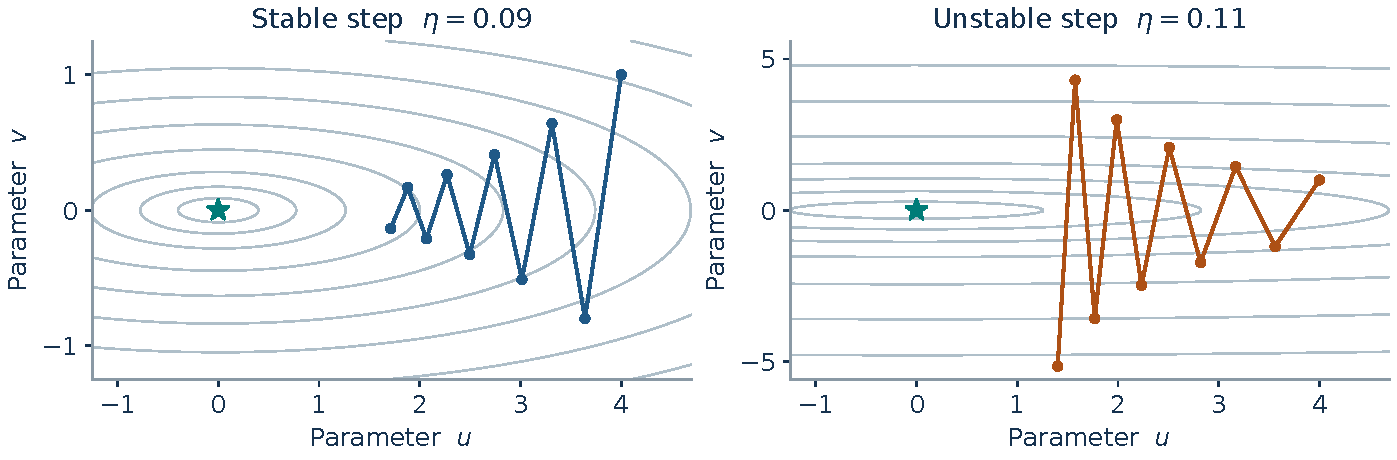
\includegraphics[width=\linewidth]{figures/ch8/valley-steps.pdf}
\caption{Nine updates from \((4,1)\) on the same loss. The star marks the
minimum. The right panel uses a wider vertical range to show the growing
oscillations.}
\end{figure}
\begin{definition}[Condition number of a positive-definite quadratic]
The Hessian is the matrix of second partial derivatives. For a quadratic
with positive-definite Hessian, define \(\kappa=c_{\max}/c_{\min}\),
where \(c_{\max}\) and \(c_{\min}\) are its largest and smallest
eigenvalues. These are the curvatures along its steepest and flattest
principal directions.
\end{definition}
In this example the Hessian is diagonal with entries \(1\) and \(20\), so
\(\kappa=20\). Stability in both directions requires \(\eta<0.1\) with
\(\eta>0\). This restriction also limits progress along the flat direction:
each stable update there keeps more than \(90\%\) of the previous value.

\clearpage
\section{Why a stochastic gradient moves at the optimum}
Return to the student model at its best fit. The predictions are still
imperfect. Compute the two derivatives separately before averaging them:
\begin{center}
\begin{tabular}{@{}rrrr@{}}\toprule
Input \(x\)& Teacher \(p_x\)& Student \(q_{a_*}(x)\)&
  \(\ell'_x(a_*)=x(q_{a_*}(x)-p_x)\)\\\midrule
1 & 0.800 & 0.6034 & \(-0.1966\)\\
2 & 0.600 & 0.6983 & \(+0.1966\)\\\bottomrule
\end{tabular}
\end{center}
Input 1 would improve if \(a\) went up. Input 2 would improve if \(a\)
went down. The two derivatives cancel at \(a_*\). If a training step sees
just one input, it takes one of those directions. For example, with
\(\eta=0.35\), the first update changes \(a\) by about \(+0.0688\) or
\(-0.0688\), each with probability \(1/2\). Either move increases the
full loss because \(a_*\) is its unique minimum.

\begin{definition}[Stochastic gradient descent]
Suppose the training loss on \(N\) examples is
\(L(w)=N^{-1}\sum_{i=1}^{N}\ell_i(w)\).
Draw an index \(I\) uniformly from \(1,\ldots,N\). A stochastic gradient
step uses \(w_{k+1}=w_k-\eta\,\nabla\ell_I(w_k)\).
\end{definition}
For fixed \(w\), each example has probability \(1/N\), so
\[
  \Expect[\nabla\ell_I(w)]
     =\frac1N\sum_{i=1}^{N}\nabla\ell_i(w)=\nabla L(w).
\]
Away from the optimum the average step points downhill. On a particular
draw the step can go uphill on the full loss, just as it did in the table.

\subsection*{What does one update cost?}
A full-gradient update uses all \(N\) example gradients. An update on
one example uses one. With a million examples, a batch of 100 permits a
parameter update after only 100 example gradients. A plot against update
number compares progress per update. To compare work as well, record the
number of examples processed or the elapsed training time.

\clearpage
\subsection*{Batch size controls the noise}
A mini-batch update uses the average of \(B\) example gradients. Hold the
parameter fixed and sample indices \(I_1,\ldots,I_B\) independently and
uniformly with replacement. Repeated indices are possible, even in the
two-input experiment.
\begin{result}[Variance of a mini-batch gradient]
Let \(g_I\) denote one component of an example gradient at the current
parameter. If its variance is \(s_g^2\), then
\[
  g_B=\frac1B\sum_{j=1}^B g_{I_j},\qquad
  \Expect[g_B]=\Expect[g_I],\qquad \Var(g_B)=s_g^2/B .
\]
\end{result}
Independence makes the variance of the sum \(B s_g^2\). The factor \(1/B\)
in the average squares to \(1/B^2\) in the variance. At \(a_*\) a single
draw gives \(+0.1966\) or \(-0.1966\), so its standard deviation is about
\(0.1966\). Averaging 16 draws reduces this to \(0.0492\). Processing
both distinct inputs once gives the exact full gradient, zero at \(a_*\).

\begin{figure}[H]\centering
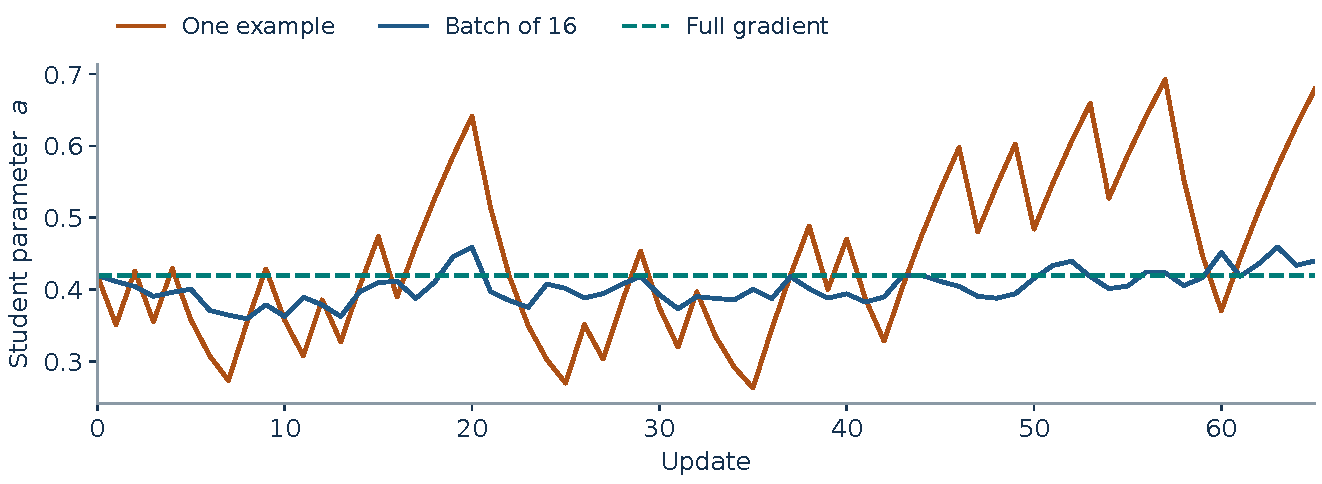
\includegraphics[width=.96\linewidth]{figures/ch8/batch-paths.pdf}
\caption{Three runs start at the same optimum and use \(\eta=0.35\).
The dashed full-gradient path stays fixed. The two sampled paths use
fresh uniform draws at each update. The blue run averages 16 draws.}
\end{figure}
The variance formula compares gradients evaluated at the \emph{same}
parameter. Once the paths separate they are evaluating different slopes.
Consequently the factor of four for gradient standard deviation does not
predict the exact ratio of spreads in a plot of parameter paths. Reducing
the learning rate also reduces the size of a random step, since the
update multiplies the sampled gradient by \(\eta\).

\clearpage
\section{Remembering past gradients}
On the narrow quadratic, successive gradients often agree along \(u\)
while alternating signs along \(v\). Consider four updates whose gradient
components along one axis are \(1,1,1,1\). Compare with \(1,-1,1,-1\)
along a second axis. An average that gives recent gradients more weight
can distinguish a persistent direction from alternating corrections.

\begin{definition}[Momentum using an exponential moving average]
Let \(g_k\) be the current full or sampled gradient. Start with \(m_0=0\);
for \(k=1,2,\ldots\), evaluate \(g_k\) at \(w_{k-1}\) and update
\[
  m_k=\beta m_{k-1}+(1-\beta)g_k,\qquad w_k=w_{k-1}-\eta m_k ,
  \qquad 0\leq\beta<1.
\]
\end{definition}
For \(\beta=1/2\), four positive gradients give averages
\(0.5,\,0.75,\,0.875,\,0.9375\). The alternating gradients give
\(0.5,\,-0.25,\,0.375,\,-0.3125\). The next step responds more strongly
to the persistent component. A moving average also takes time to reverse
after a genuine change of direction, so momentum can overshoot.

\begin{figure}[H]\centering
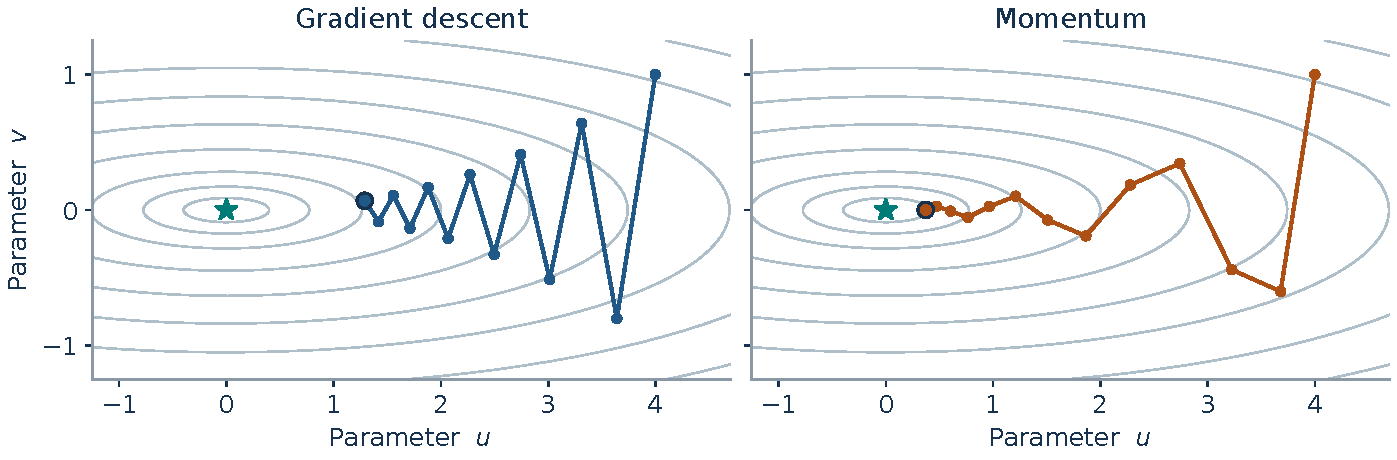
\includegraphics[width=\linewidth]{figures/ch8/momentum.pdf}
\caption{Twelve updates on the same contours from \((4,1)\). The larger
dot is the last iterate and the star is the minimum. Left: gradient
descent with \(\eta=0.09\). Right: momentum with \(\beta=0.5\) and
\(\eta=0.16\) in the moving-average convention above.}
\end{figure}
The settings illustrate how the two methods move. The learning rate is
part of each method's configuration. For a speed comparison, tune it for
each method, then compare the cost of reaching the same target loss.

\clearpage
\section{How Adam scales a step}
Suppose one parameter repeatedly receives gradients of size 10 while
another receives gradients of size \(0.1\). Momentum keeps track of their
directions, but their typical magnitudes still differ by a factor of 100.
Adam also tracks the squared gradients of each parameter. Their running
averages provide a local scale for the update.

\begin{definition}[Adam]
Write the equations for one parameter; apply them separately to each
coordinate of a vector. Let \(g_k\) be its gradient at step \(k\ge1\).
Start with \(m_0=s_0=0\) and choose \(0\le\beta_1,\beta_2<1\).
\begin{align*}
 m_k &=\beta_1m_{k-1}+(1-\beta_1)g_k,&
 s_k &=\beta_2s_{k-1}+(1-\beta_2)g_k^2,\\
 \widehat m_k&=m_k/(1-\beta_1^k),&
 \widehat s_k&=s_k/(1-\beta_2^k).
\end{align*}
The step is \(w_k=w_{k-1}-\eta\,\widehat m_k/(\sqrt{\widehat s_k}+\varepsilon)\),
where \(\varepsilon>0\) keeps the denominator positive.
\end{definition}
The correction factors account for starting both averages at zero. On the
first update, \(m_1=(1-\beta_1)g_1\), so \(\widehat m_1=g_1\);
likewise \(\widehat s_1=g_1^2\). For a first gradient \(g_1=10\), the
ratio in the update is \(10/(10+\varepsilon)\). For \(g_1=0.1\), it is
\(0.1/(0.1+\varepsilon)\). Both are close to one for sufficiently small
\(\varepsilon\). Later steps depend on the history of each coordinate.
The second moving average estimates a raw second moment; opposing
gradients can have a small average and a large average square.

\subsection*{Reading a training curve}
In the student model, a single-example step away from \(a_*\) increases
the full loss even when the derivative is correct. Averaging all example
gradients at that point makes the update zero. On the quadratic, a
full-gradient run with \(\eta=0.11\) diverges whenever its starting \(v\)
is nonzero. It already uses every example. Here reducing the step below
\(0.1\) restores stability.

\smallskip
{\small\textbf{Further reading.}
\href{https://introml.mit.edu/_static/spring23/LectureNotes/6_390_lecture_notes_spring23.pdf}{MIT 6.390, Chapter 3} develops gradient descent and SGD.
\href{https://www.cs.cornell.edu/courses/cs4787/2026fa/lectures/lecture6.html}{Cornell CS4787, Lecture 6} analyzes step size and batch size on quadratics.
\href{https://cs231n.stanford.edu/slides/2025/lecture_3.pdf}{Stanford CS231n, Lecture 3, slides 56--75} illustrates momentum and adaptive updates.}
